\documentclass[12pt,a4paper,twoside]{article}
\usepackage{amsmath}
\usepackage{amssymb}
\usepackage{amsthm}
\usepackage{array}
\usepackage{amsfonts}
\usepackage{ctable,booktabs}
%\usepackage[pdftex]{graphicx}
\usepackage{enumerate}
\usepackage{fancyhdr}
\usepackage{float}
\usepackage{fullpage}
\usepackage[margin=1in]{geometry}
\usepackage{mathrsfs}%Math script
\usepackage{sidecap}
\usepackage{tabularx} 
\usepackage{verbatim}
\usepackage{wrapfig}
\usepackage[all,cmtip]{xy}%Commutative diagrams
	\headheight 0cm
	\setlength{\headsep}{18pt}
	\setlength{\headheight}{15.2pt}

\newtheoremstyle{norm}
{3pt}
{3pt}
{}
{}
{\bf}
{:}
{.5em}
{}

\theoremstyle{norm}
\newtheorem{thm}{Theorem}[section]
\newtheorem{lem}[thm]{Lemma}
\newtheorem{df}[thm]{Definition}
\newtheorem{rem}[thm]{Remark}
\newtheorem{st}{Step}
\newtheorem{pr}[thm]{Proposition}
\newtheorem{cor}[thm]{Corollary}
\newtheorem{conj}[thm]{Conjecture}
\newtheorem{clm}[thm]{Claim}
\newtheorem{exr}[thm]{Exercise}
\newtheorem{ex}[thm]{Example}
\newtheorem{prb}[thm]{Problem}

%Math blackboard, fraktur, and script commonly used letters
\newcommand{\A}[0]{\mathbb{A}}
\newcommand{\C}[0]{\mathbb{C}}
\newcommand{\sC}[0]{\mathcal{C}}
\newcommand{\cE}[0]{\mathscr{E}}
\newcommand{\F}[0]{\mathbb{F}}
\newcommand{\cF}[0]{\mathscr{F}}
\newcommand{\sF}[0]{\mathscr{F}}
\newcommand{\cG}[0]{\mathscr{G}}
\newcommand{\sH}[0]{\mathscr H}
\newcommand{\Hq}[0]{\mathbb{H}}
\newcommand{\N}[0]{\mathbb{N}}
\newcommand{\Pj}[0]{\mathbb{P}}
\newcommand{\sO}[0]{\mathcal{O}}
\newcommand{\cO}[0]{\mathscr{O}}
\newcommand{\Q}[0]{\mathbb{Q}}
\newcommand{\R}[0]{\mathbb{R}}
\newcommand{\Z}[0]{\mathbb{Z}}
%Lowercase
\newcommand{\ma}[0]{\mathfrak{a}}%ideal a
\newcommand{\mb}[0]{\mathfrak{b}}
\newcommand{\fg}[0]{\mathfrak{g}}
\newcommand{\vi}[0]{\mathbf{i}}%vector i
\newcommand{\vj}[0]{\mathbf{j}}
\newcommand{\vk}[0]{\mathbf{k}}
\newcommand{\mm}[0]{\mathfrak{m}}%ideal m
\newcommand{\mfp}[0]{\mathfrak{p}}
\newcommand{\mq}[0]{\mathfrak{q}}
\newcommand{\mr}[0]{\mathfrak{r}}
%More sequences of letters
\newcommand{\fq}[0]{\mathbb{F}_q}
\newcommand{\fqt}[0]{\mathbb{F}_q^{\times}}
\newcommand{\sll}[0]{\mathfrak{sl}}
%Shortcuts for symbols
\newcommand{\nin}[0]{\not\in}
\newcommand{\opl}[0]{\oplus}
\newcommand{\ot}[0]{\otimes}
\newcommand{\rc}[1]{\frac{1}{#1}}
\newcommand{\sub}[0]{\subset}
\newcommand{\subeq}[0]{\subseteq}
\newcommand{\supeq}[0]{\supseteq}
\newcommand{\nsubeq}[0]{\not\subseteq}
\newcommand{\nsupeq}[0]{\not\supseteq}
%Arrows
\newcommand{\lar}[0]{\leftarrow}
\newcommand{\ra}[0]{\rightarrow}
\newcommand{\rra}[0]{\rightrightarrow}
\newcommand{\hra}[0]{\hookrightarrow}
\newcommand{\send}[0]{\mapsto}
%Shortcuts for greek letters
\newcommand{\al}[0]{\alpha}
\newcommand{\be}[0]{\beta}
\newcommand{\ga}[0]{\gamma}
\newcommand{\Ga}[0]{\Gamma}
\newcommand{\de}[0]{\delta}
\newcommand{\ep}[0]{\varepsilon}
\newcommand{\eph}[0]{\frac{\varepsilon}{2}}
\newcommand{\ept}[0]{\frac{\varepsilon}{3}}
\newcommand{\la}[0]{\lambda}
\newcommand{\La}[0]{\Lambda}
\newcommand{\ph}[0]{\varphi}
\newcommand{\rh}[0]{\rho}
\newcommand{\te}[0]{\theta}
\newcommand{\om}[0]{\omega}
\newcommand{\Om}[0]{\Omega}
%Brackets
\newcommand{\ab}[1]{\left| {#1} \right|}
\newcommand{\an}[1]{\langle {#1}\rangle}
\newcommand{\ba}[1]{\left[ {#1} \right]}
\newcommand{\bc}[1]{\left\{ {#1} \right\}}
\newcommand{\ce}[1]{\left\lceil {#1}\right\rceil}
\newcommand{\fl}[1]{\left\lfloor {#1}\right\rfloor}
\newcommand{\pa}[1]{\left( {#1} \right)}
%Text
\newcommand{\btih}[1]{\text{ by the induction hypothesis{#1}}}
\newcommand{\bwoc}[0]{by way of contradiction}
\newcommand{\by}[1]{\text{by~(\ref{#1})}}
\newcommand{\ore}[0]{\text{ or }}
\newcommand{\wog}[0]{ without loss of generality }
\newcommand{\Wog}[0]{ Without loss of generality }
%Functions, etc.
\newcommand{\Ann}{\operatorname{Ann}}
\newcommand{\AP}{\operatorname{AP}}
\newcommand{\Ass}{\operatorname{Ass}}
\newcommand{\chr}{\operatorname{char}}
\newcommand{\cis}{\operatorname{cis}}
\newcommand{\Cl}{\operatorname{Cl}}
\newcommand{\Der}{\operatorname{Der}}
\newcommand{\End}{\operatorname{End}}
\newcommand{\Ext}{\operatorname{Ext}}
\newcommand{\Frac}{\operatorname{Frac}}
\newcommand{\FS}{\operatorname{FS}}
\newcommand{\GL}{\operatorname{GL}}
\newcommand{\Hom}{\operatorname{Hom}}
\newcommand{\chom}[0]{\mathscr{H}om}
\newcommand{\Ind}[0]{\text{Ind}}
\newcommand{\im}[0]{\text{im}}
\newcommand{\nil}[0]{\operatorname{nil}}
\newcommand{\Proj}{\operatorname{Proj}}
\newcommand{\Rad}{\operatorname{Rad}}
\newcommand{\Res}[0]{\text{Res}}
\newcommand{\sign}{\operatorname{sign}}
\newcommand{\SL}{\operatorname{SL}}
\newcommand{\Spec}{\operatorname{Spec}}
\newcommand{\Specf}[2]{\Spec\pa{\frac{k[{#1}]}{#2}}}
\newcommand{\spp}{\operatorname{sp}}
\newcommand{\spn}{\operatorname{span}}
\newcommand{\Supp}{\operatorname{Supp}}
\newcommand{\Tor}{\operatorname{Tor}}
\newcommand{\tr}[0]{\text{Tr}}
%Commutative diagram shortcuts
\newcommand{\commsq}[8]{\xymatrix{#1\ar[r]^{#6}\ar[d]^{#5} &#2\ar[d]^{#7} \\ #3 \ar[r]^{#8} & #4}}
%Makes a diagram like this
%1->2
%|    |
%3->4
%Arguments 5, 6, 7, 8 on arrows
%  6
%5  7
%  8
\newcommand{\pull}[9]{
#1\ar@/_/[ddr]_{#2} \ar@{.>}[rd]^{#3} \ar@/^/[rrd]^{#4} & &\\
& #5\ar[r]^{#6}\ar[d]^{#8} &#7\ar[d]^{#9} \\}
\newcommand{\back}[3]{& #1 \ar[r]^{#2} & #3}
%Syntax:\pull 123456789 \back ABC
%1=upper left-hand corner
%2,3,4=arrows from upper LH corner, going down, diagonal, right
%5,6,7=top row (6 on arrow)
%8,9=middle rows (on arrows)
%A,B,C=bottom row
%Other
\newcommand{\op}{^{\text{op}}}
\newcommand{\fp}[1]{^{\underline{#1}}}%Falling power
\newcommand{\rp}[1]{^{\overline{#1}}}
\newcommand{\rd}[0]{_{\text{red}}}
\newcommand{\pre}[0]{^{\text{pre}}}
\newcommand{\pf}[2]{\pa{\frac{#1}{#2}}}%Shortcut for fraction with parentheses
\newcommand{\pd}[2]{\frac{\partial #1}{\partial #2}}%Partial derivatives
%Matrices
\newcommand{\coltwo}[2]{
\left[
\begin{array} {c}
{#1}\\
{#2} 
\end{array}
\right]}
\newcommand{\matt}[4]{
\begin{pmatrix} {cc}
{#1}&{#2}\\
{#3}&{#4}
\end{pmatrix}
}
\newcommand{\smatt}[4]{
\left[\begin{smallmatrix} {cc}
{#1}&{#2}\\
{#3}&{#4}
\end{smallmatrix}\right]
}
\newcommand{\colthree}[3]{
\begin{pmatrix} {c}
{#1}\\
{#2}\\
{#3}
\end{pmatrix}
}
%Page breaks in equations
\allowdisplaybreaks[1]

\rhead{\qquad}
%\lhead{}\rhead{}\cfoot{}\chead{} 
%\lfoot[\fancyplain{}{\bfseries\thepage}]{}
%\rfoot[]{\thepage}
%\lfoot[\thepage]{}

%\setlength{\oddsidemargin}{0.55in}
%\setlength{\evensidemargin}{0.55in}


%\fi
\pagestyle{fancy}

%OMC <year>
\lhead{\textit{OMC 2011}}

% LECTURE TITLE
\chead{Generating functions}

%%%%%%%%%%
% LECTURE NUMBER
%%%%%%%%%%
\rhead{\textit{Lecture 18}}


%%%%%%%%%%
% CONTENT
%
% Here is where you place the problems and any other content. If you are making a problem set, use the \item command to create a new problem. 
%
%%%%%%%%%%
\begin{document}
\title{Lecture $18$ --- Generating functions}% !! Remember to change the lecture number
\author{Holden Lee}
\date{4/23/11}% !! Remember to change the date
\maketitle
\thispagestyle{empty}
\section{Introduction}\label{intro}
Generating functions offer a way to convert combinatorics questions into purely algebraic and analytic questions. The basic idea is this: we take a sequence $a_0,a_1,a_2,\ldots $, usually representating something of combinatorical interest---for example, $a_n$ could be the number of ways to make change with $n$ cents (see the first lecture)---and then associate with it a power series.
\begin{df}
The \textbf{generating function} of the sequence $a_0,a_1,a_2,\ldots$ is the {\it formal series}
\[
\sum_{n=0}^{\iy} a_nx^n=a_0+a_1x+a_2x^2+\cdots.
\]
\end{df}
To find the $a_n$, or identities involving the $a_n$, we rewrite the generating function in terms of familiar functions using algebra and calculus, manipulate the equation, and then extract the coefficients.

In Sections~\ref{formal} we develop the algebraic and analytic machinery of generating functions; in Sections~\ref{alg} and~\ref{comb} we give applications to algebra and combinatorics. %l look at generating functions from an algebraic and analytic (i.e. calculus) perspective. 
An impatient reader may also wish to skip to the examples, and look up the relevant algebraic and analytic facts as needed.

In our above definition, we said that a generating function is a {\it formal series}. But what exactly is a formal series?
\section{Formal series}\label{formal}
\subsection{The ring of formal series}
\begin{df}
Let $R$ be a ring. The \textbf{ring of formal (power) series} in $R$ is the set of all expressions
\[
\sum_{n=0}^{\iy} a_nx^n=a_0+a_1x+a_2x^2+\cdots.
\]
The ring of formal series will be denoted by $R[[x]]$ (compare to the ring of polynomials $R[x]$). 
\end{df}
We will work exclusively with $R=\R$, i.e. formal series with real coefficients. Just like polynomials, we can repeat this process to obtain formal series in more than one variable, to get $R[[x]][[y]]=R[[x,y]]$, etc.

Note a formal series is {\it not} a function. Right now we don't care whether the sum $\sum_{n=0}^{\iy} a_nx^n$ ``converges." Don't think of $x$ as being the input value for a function; think of it just as the symbol $x$. Note this perspective was useful in our development of polynomials; it will also be essential for our development of formal series. (In Section~\ref{calc} we {\it will} look at formal series as functions.)

We said $R$ is a ring, meaning that it has addition and multiplication defined, satisfying the ``usual" properties (see lecture 8). If $f$ and $g$ are power series, we define $f+g$ by adding corresponding terms and multiplication by multiplying every term in $f$ and every term in $g$, and adding. In symbols, if
\begin{align*}
f(x)&=\sum_{n=0}^{\iy} a_n x^n\\
g(x)&=\sum_{n=0}^{\iy} b_n x^n
\end{align*}
then
\begin{align}
\nonumber
f(x)+g(x)&=\sum_{n=0}^{\iy} (a_n+b_n)x^n\\
f(x)g(x)&=\sum_{n=0}^{\iy} (a_nb_0+a_{n-1}b_1+\cdots +a_1b_{n-1}+a_0b_n)x^n.\label{prod}
\end{align}
Note that the coefficient of $fg$ is the sum of products of coefficients in $f$ and coefficients in $g$, where the corresponding exponents sum to $n$.\footnote{The sequence of coefficients of $f(x)g(x)$ is called the {\it convolution} of $\{ a_n\}$ and $\{b_n\}$.} This generalizes to the product of $m$ factors in the obvious way (for 3 sequences $f(x)g(x)h(x)=\sum_{i+j+k=n} a_ib_jc_kx^n$, and so on), and will be important for combinatorial interpretations.

It is simple to check that we have additive inverses and that the normal rules distributivity, commutativity, and associativity hold. We will leave this for the fastidious reader.

There is one more thing we could do: we can compose power series, that is, substitute one in for the other.
\begin{df}
Given $f(x)=\sum_{n=0}^{\iy} a_n x^n$ and $g(x)=\sum_{n=1}^{\iy} b_n x^n$, define the \textbf{composition} $f\circ g$ to be
\[
f\circ g(x)=\sum_{n=0}^{\iy}a_n g(x)^n.
\]
\end{df}
Note this makes sense, because for $n>0$, the coefficient of $x^n$ in $f\circ g$ will only depend on the partial sum $\sum_{m=0}^{n} a_mg(x)^m$ (why?). Note that we require the constant term of $g$ to be 0 to avoid an infinite sum for the constant term. This way, the constant term of $f\circ g$ equals $a_0$, the constant term of $f$.
\subsection{Inverses}
If $f$ is a power series, a logical question is whether $\rc{f}$ or $f^{-1}$ is well-defined. You may know the geometric series formula,
\[
\rc{1-x}=1+x+x^2+x^3+\cdots
\]
which says that $1+x+x^2+\cdots $ is the multiplicative inverse of $\rc{1-x}$ in $\R[[x]]$. Indeed you can check using our definition of multiplication that $(1-x)(1+x+x^2+\cdots )=1$. Now we see under what conditions $\rc{f}$ and $f^{-1}$ exist.
\begin{thm}\label{multinv}
Suppose $f=\sum_{n=0}^{\iy}a_n x^n$ where $a_0\neq 0$. Then there exists a unique $g$ such that $fg=1$. $g$ is called the \textbf{multiplicative inverse} of $f$ and denoted by $\rc{f}$.

Moreover, the coefficient of $x^n$ in $g$ only depends on $a_0,\ldots, a_n$.
\end{thm}
\begin{proof}
We find the coefficients $b_0,b_1,\ldots$ of $g$ inductively. To make the constant term 1 we need $b_0=\rc{a_0}$.

Suppose we know that $g$ starts with $b_0+b_1x+\cdots+b_kx^k$ and $f(x)(b_0+b_1x+\cdots+b_kx^k)$ has coefficients of $1,x,\ldots, x^k$ all equal to 0. Now we define $b_{k+1}$ so that the coefficients of $1,x,\ldots, x^{k+1}$ in $f(x)(b_0+b_1x+\cdots+b_kx^k+b_{k+1}x^{k+1})$ are equal to 0. The coefficients of $1,x,\ldots, x^k$ are not affected by the addition of $b_{k+1}x^{k+1}$, so we just need the coefficient of $x^{k+1}$ to be 0:
\[
a_0b_{k+1}+a_1b_k+\cdots +a_{k+1}b_0=0.
\]
So let
\[
b_{k+1}=\frac{-a_1b_k-\cdots -a_{k+1}b_0}{a_0},
\]
and this is the only value that works.

Then $g=\sum_{n=0}^{\iy} b_n x^n$.
\end{proof}
\begin{thm}
Suppose $f=\sum_{n=1}^{\iy} a_nx^n$. Then there exists a unique $g$ such that $f\circ g=1$. Moreover, $g\circ f$ as well. $g$ is called the  %\textbf{compositional inverse} or simply 
\textbf{inverse} of $f$ and denoted by $f^{-1}$.

Moreover, the coefficient of $x^n$ in $g$ depends only on $a_1,\ldots, a_n$.
\end{thm}
\begin{proof}
Exercise. (Similar to the above proof.)
\end{proof}
%\subsection{Laurent series}
%We can also allow negative coefficients in formal series.
%\begin{df}
%The \textbf{ring of formal Laurent series} in the ring $R$ is the set of all expressions
%\[
%\sum_{n\in \Z}a_nx^n
%\]
%where only a {\it finite} number of the $a_n$ are nonzero when $n$ is negative. The ring of formal Laurent series is denoted by $R((x))$.
%\end{df}
%All the properties carry over, with summation now carried out over all integers. The only change is that now all series have multiplicative inverses, not just series with constant term nonzero.

\subsection{Derivatives}
We define the derivative the same way as in calculus.
\begin{df}
Let $f(x)=\sum_{n=0}^{\iy} a_nx^n$. The \textbf{derivative} of $f$ is 
\[
f'(x)=\sum_{n=1}^{\iy} na_nx^{n-1}=\sum_{n=0}^{\iy} (n+1)a_{n+1}x^n.
\]
\end{df}
The following can be proved just like it is proved for polynomials. (Alternatively, conclude it from the corresponding result for polynomials, by noting that the coefficients of $x^n$ depends on only finitely many terms in the expressions below.)
\begin{pr}
Let $f,g$ be two power series and $c$ be a constant. Then
\begin{enumerate}
\item (Linearity) 
$(cf+g)'=cf'+g'$.
\item (Product rule)
$(fg)'=f'g+fg'$.
\item (Chain rule) For $g$ with constant term 0, 
$(f\circ g)'=(f'\circ g)g'$.
\end{enumerate}
\end{pr}
We can state the product rule in a slightly different form, that will often be of use.
\begin{pr}[Logarithmic differentiation]\label{logdiff}
Suppose $f=f_1\cdots f_n$ where $f_1,\ldots, f_n$ are power series. Then
\[
f'=f\pa{\frac{f_1'}{f_1}+\cdots +\frac{f_n'}{f_n}}.
\]
\end{pr}
\begin{proof}
By the product rule,
\[f'=f_1'f_2\cdots f_n+f_1f_2'\cdots f_n+\cdots +f_1f_2\cdots f_n'.\]
which gives the above after using $f=f_1\cdots f_n$.

Alternatively (and this is why the proposition is called logarithmic differentiation) take ln of both sides, differentiate, and use the chain rule, and note that $(\ln x)'=\rc{x}$:
\begin{align}
\nonumber \ln f&=\ln f_1+\ln f_2+\cdots +\ln f_n\\
\label{log2} \frac{f'}{f}&=\frac{f_1'}{f_1}+\frac{f_2'}{f_2}+\cdots +\frac{f_n'}{f_n}
\end{align}
which rearranges into the same identity.

Why is this justified? This identity is true if the $f_i$'s are all polynomials, by calculus and Theorem~\ref{calctoform} in the next subsection. Moreover, the coefficient of $x^n$ on both sides of~(\ref{log2}) will stay the same if each $f,f_i$ is replaced by a polynomial with coefficients of $1,x,\ldots, x^{n+1}$ agreeing (so the coefficients of $1,\ldots, x^n$ of $f_1',\ldots, f_n'$ will be the same; use the last statement in Theorem~\ref{multinv}), so the conclusion follows from the finite case.
\end{proof}
\subsection{Analytic point of view}\label{calc}
From calculus, we know how to expand functions in power series $\sum_{n=0}^{\iy}a_nx^n$. For each power series there is a $r$ such that it converges absolutely\footnote{That is, $\sum_{n=0}^{\iy} |a_nx^n|$ is finite.} for $|x|<r$, but not for $|x|>r$. In this domain we may differentiate and integrate and still have a convergent power series. 

A table of power series and generating functions can be found in the Appendix. For example,
\[
e^x=1+\frac{x}{1!}+\frac{x^2}{2!}+\cdots.
\]
We have equality in the {\it calculus} sense: both sides are equal as functions, i.e. give the same result when we plug in any value for $x$.

An identity in formal power series automatically transfers to an identity in functions, provided the functions converge. The following gives the opposite implication.
\begin{thm}\label{calctoform}
Suppose $f(x)=\sum_{n=0}^{\iy} a_nx^n$ and $g(x)=\sum_{n=0}^{\iy} b_nx^n$ are two absolutely convergent power series on an interval $(-\ep,\ep)$ around 0, and $f(x)=g(x)$ for $x\in (-\ep,\ep)$. Then $a_n=b_n$ for all $n$.
\end{thm}
\begin{proof}
Let $h(x)=f(x)-g(x)=\sum_{n=0}^{\iy} c_nx^n$, where $c_n=a_n-b_n$. If $c_n$ is not the zero sequence, let $m$ be the least integer so that $c_m\ne 0$. Then $h(x)=x^m(c_m+j(x))$ where $j(x)=c_{m+1}x+c_{m+2}x^2+\cdots$. Since power series are continuous, $j(x)$ is continuous. Note it equals 0 at $x=0$, so is close to 0 for $x$ close to 0. Taking $x\ne 0$ sufficiently small, we have $|j(x)|<|a_m|$, so $a_m+j(x)\ne 0$ and $h(x)\ne 0$, contradiction.
\end{proof}
As a simple example, we know
\[
\rc{1-x}=1+x+x^2+x^3+\cdots
\]
holds for $x\in (-1,1)$, so this is an identity of power series. (Recall we could also conclude this by directly multiplying $(1-x)$ and $1+x+x^2+\cdots$.)

Why is calculus useful?
\begin{enumerate}
\item It allows us to turn power series into familiar functions, which we can easily multiply, divide, and differentiate, taking full advantage of algebraic identities (ex. $\sin^2x+\cos^2x=1$---it would be annoying to the corresponding power series satisfy this identity using the definition of multiplication for formal series!).
\item It allows us to substitute in values for $x$ to get identities involving the coefficients, or take limits (see Section~\ref{arith}).
\item We could the tools of complex analysis to analyze the growth of the sequence. (This is beyond the scope of this lecture.)
\end{enumerate}
\section{Applications to Algebra}\label{alg}
We give two applications of generating functions to algebra.
First, generating functions are useful for finding closed formulas for sequences. The general strategy is the following.
\begin{enumerate}
%\item Find a recurrence relation for the sequence.
\item Convert the recurrence relation for $a_n$ into an identity involving the generating function $f$.
\begin{enumerate}
\item Shift the sequence by multiplying by powers of $x$. For fixed $i$, the generating function for $a_{n-i}$ is $f(x)x^i$; the generating function of $a_{n+i}$ is $x^{-i}(f(x)-a_0-\cdots -a_{i-1}x^{i-1})$.
\item The sequence $(n+1)a_{n+1}$ is obtained by taking the derivative of $f$.
\item A term like $a_nb_0+\cdots+a_0b_n$ is obtained by multiplying power series.
\end{enumerate}
\item If we want a closed formula for the sequence, solve for $f$ and extract the coefficients.

If we want to prove an identity or simplify and expression involving the sequence, massage the identity for $f$ so that the desired identity can be read off from equating coefficients of $x^n$.
\end{enumerate}
%Item 1 is important when we deal with combinatorics problems, in the next section. Here, we will be given a recurrence relation, and we will carry out steps 2-3.
\subsection{Solving recurrences}
\begin{thm}
%Simple version
Suppose that $c_0\ne 0$ and the roots of $P(x):=x^{k}+c_{k-1}x^{k-1}+\cdots +c_1x+c_0=0$ are distinct and equal to $r_1,\ldots, r_k$. 
The general solution to the linear recurrence
\[
a_n+c_{k-1}a_{n-1}+\cdots +c_0a_{n-k}=0,\,n\ge k
\]
where $c_0\ne 0$, is 
\begin{equation}\label{gensoln}
a_n=b_1r_1^n+b_2r_2^n+\cdots +b_kr_k^n.
\end{equation}
%General version. A bit more complicated.
%The general solution to the linear recurrence
%\[
%a_n+c_{k-1}a_{n-1}+\cdots +c_0a_{n-k}=0,\,n\ge k
%\]
%where $c_0\ne 0$, 
%is given by
%\[
%a_n=\sum_{r}P_r(x)r^n
%\]
%where the sum is over the roots $r$ of the characteristic polynomial $x^k+c_{k-1}x^{k-1}+\cdots +c_0$ and $P_r(x)$ is a polynomial of degree less than $\text{mult}_P(r)$, the multiplicity of the root $r$ in $P$.
\end{thm}
\begin{proof}
Let $f(x)$ be the generating function for $a_n$, so that $f(x)=\sum_{n=0}^{\iy} a_n x^n$. We multiply $f(x)$ by powers of $x$ to get the shifted sequences $\{a_{n-i}\}$:
\[
x^if(x)=\sum_{n=0}^{\iy} a_n x^{n+i}=\sum_{n=i}^{\iy} a_{n-i} x^n.
\]
Thus the recurrence relation becomes
\[
f(x)+c_{k-1}xf(x)+\cdots +c_0x^kf(x)=0,
\]
because the coefficient of $x^n$ on left hand side is $a_n+c_{k-1}a_{n-1}+\cdots +c_0a_{n-k}$, which is equal to 0. Dividing by $1+c_{k-1}x+\cdots +c_0x^k$, we obtain $f(x)=0$. Wait, that's not right. What went wrong?

The identity $a_n+c_{k-1}a_{n-1}+\cdots +c_0a_{n-k}=0$ is only valid for $n\ge k$. (Moral: always be careful with small cases.) So for $n<k$, there is no restriction on the coefficient of $x^n$ on the LHS. So instead, we should write
\begin{equation}\label{linrec}
f(x)+c_{k-1}xf(x)+\cdots +c_0x^kf(x)=d_0+d_1x+\cdots +d_{k-1}x^{k-1}
\end{equation}
for some $b_0,\ldots, b_{k-1}$. Now we use the following:
\begin{thm}[Partial fraction decomposition]
Suppose $p(x)$ and $q(x)$ are polynomials with $\deg p<\deg q=k$, and $q$ has distinct roots $r_1,\ldots, r_n$. Then there are $b_1,\ldots, b_k$ such that
\[
\frac{p(x)}{q(x)}=\frac{b_1}{x-r_1}+\cdots +\frac{b_k}{x-r_k}.
\]
%General version
%Then there are (unique) polynomials $f_r(x)$ with $\deg f_r<\text{mult}_q(r)$ such that
%\[
%\frac{p(x)}{q(x)}=\sum_{r} \frac{f_r(x)}{(x-r)^{\text{mult}_q(r)}}.
%\]
\end{thm}
Hence dividing~(\ref{linrec}) by $1+c_{k-1}x+\cdots +c_0x^k$, noting that $\rc{r_i}$ are the zeros of $1+c_{k-1}x+\cdots +c_0x^k=x^nP\pf{1}{x^n}$, and using the above theorem gives
\begin{align*}
f(x)&=\frac{b_1}{x-\rc{r_1}}+\cdots +\frac{b_k}{x-\rc{r_k}}\\
&=\frac{-r_1b_1}{1-r_1x}+\cdots +\frac{-r_nb_n}{1-r_nx}.
\end{align*}
for some $b_i$. 
(Conversely, given $f(x)$ in the above form,~(\ref{linrec}) holds for some $b_i$, so $f(x)$ gives a valid sequence.) 
Now using the geometric series formula gives
\[
f(x)=\sum_{i=1}^k -r_ib_i(1+r_ix+r_i^2x^2+r_i^3x^3+\cdots ).
\]
Extracting the $n$th coefficient gives
\[
a_n=\sum_{i=1}^k -r_ib_i r_i^n=\sum_{i=1}^kb_i'r_i^n
\]
after setting $b_i'=-r_ib_i$.
\end{proof}
\begin{rem}
In the general case, the general solution to the linear recurrence
\[
a_n+c_{k-1}a_{n-1}+\cdots +c_0a_{n-k}=0,\,n\ge k
\]
where $c_0\ne 0$, 
is given by
\[
a_n=\sum_{r}P_r(x)r^n
\]
where the sum is over the roots $r$ of the characteristic polynomial $x^k+c_{k-1}x^{k-1}+\cdots +c_0$ and $P_r(x)$ is a polynomial of degree less than the multiplicity of the root $r$ in $P$. The above proof can be adapted to solve the general version.
\end{rem}
Note that generating sequences do not necessarily make for the most elegant or short proofs. If we know the general form of the solution, we can prove show that it works just by substituting in, and find an argument to show directly that all solutions are of that form. But generating sequences are especially useful if we do not know the solution, since they offer a methodical way to find it. For some deep results, though, no proof without generating functions is known!
\subsection{Newton sums}
Let $ x_1,x_2,\ldots$ be variables. In this subsection we develop the Newton formulas relating the symmetric polynomials in the $ x_i$
\[s_n=\sum_{1\leq i_1<\cdots <i_n}x_{i_1}x_{i_2}\cdots x_{i_n}\]
and the power sums
\[p_n=\sum_{i\geq 1} x_i^n.\]

(For example, when we have 3 variables, $ s_2=x_1x_2+x_1x_3+x_2x_3$ and $ p_2=x_1^2+x_2^2+x_3^2$. For convenience of notation we don't restrict the number of variables; if we are working with $ k$ variables we could just set $ 0=x_{k+1}=x_{k+2}=\cdots $. By convention $ s_0=1$.)

We note that the $s_i$ and $p_i$ are the coefficients of powers of $ t$ of the following generating functions.
\begin{align*} S(t)&=\prod_{i\geq 1} (1+x_it)=1+s_1t+s_2t^2+\cdots\\
P(t)&=\sum_{i\geq 1}\frac{x_i}{1-x_it}=\sum_{i\geq 1} (x_i+x_i^2t+\cdots)=p_1+p_2t+\cdots.
\end{align*}
Why do these expansions hold? Each term in the expansion of $ S(t)$ is a term of the form $ x_{i_1}\cdots x_{i_n}t^n$ where the $ x_{i_j}$ are distinct, since we can only get a factor of $ x_{i_j}$ from the factor $ (1+x_{i_j}t)$. Since each $ x_i$ always comes with a factor of $ t$, $ t$ acts as a ``counter" giving the total number of variables. Grouping the terms with $ t^n$ we get all combinations of products of $ n$ of the $ x_i$.

For $ P(t)$ the argument is simpler: expand in geometric series as shown above to get that the coefficients of $ t^{n-1}$ are the $ n$th powers of the $ x_i$.

We want an identity involving $ s_i$ and $ p_i$ so we look for an identity involving $ S(t)$ and $ P(t)$. First we turn the $ 1+xt_i$ into $ 1-x_it$: define
\[\Psi(t)=S(-t)=\prod_{i\geq 1} (1-x_it)=1-s_1t+s_2t^2-s_3t^3+\cdots.\]
Now use logarithmic differentiation (Proposition~\ref{logdiff}) to get
%$ \displaystyle \ln(\Psi(t))=\sum_{i\geq 1} \ln(1-x_it).$
%Now differentiate both sides.
\[\frac{\Psi'(t)}{\Psi(t)}=-\sum_{i\geq 1} \frac{x_i}{1-x_it}.\]
The right-hand side is just $ -P(t)$ (TA-DA!). Thus we get
\[ -\Psi'(t)=\Psi(t)P(t).\]
Now we match coefficients of $ t^{n-1}$ on both sides. Note
\[ -\Psi'(t)=s_1-2s_2t+3s_3t^2-\cdots\]
so the coefficient of $ t^{n-1}$ is $ (-1)^{n+1}n s_n$. To get the coefficients of the right-hand side, note that a term containing $ t^{n-1}$ on the RHS comes from multiplying $ (-1)^is_it^i$ in $ \Psi(t)$ and a term $ p_{n-i}t^{n-i-1}$ in $ P(t)$. Thus the coefficients of $ t^{n-1}$ are
\[ (-1)^{n+1}ns_n=\sum_{i=0}^{n-1}(-1)^is_ip_{n-i}=s_0p_n-s_1p_{n-1}+\cdots +(-1)^{n-1}s_{n-1}p_1\]
which is the Newton sum formula.

\section{Applications to Combinatorics}\label{comb}
%\begin{thm}
%Suppose $f_i(x)=\sum_{n=0}^{\iy} a_{i,n}x^n$, and there are 
%\end{thm}
In some combinatorial problems, we find a recurrence relation for the sequence of interest, and then turn it into a generating series (see Section~\ref{catalan}). In others, we build the generating function directly by multiplying together several power series, and note that every resulting term is obtained by choosing one term from each of the series; the exponents of the variable acts should like some ``weight," or some value of interest to the problem. (See Theorem~\ref{partitiongf} and Example~\ref{imo95-6}.)

See also the first lecture (\url{http://onlinemathcircle.com/wp-content/uploads/2010/12/1-beauty.pdf}) for an application of generating functions to counting change.

\subsection{Binomial coefficients}
By the binomial formula,
\[
(1+x)^n=\sum_{i=0}^n \binom ni x^n.
\]
Thus $(1+x)^n$ is the generating function for the sequence $\binom ni, i\ge 0$. This is a particularly simple function; in fact is is just a polynomial! We can use this and our knowledge of multiplying generating functions (or just polynomials) to get a quick identity.
\begin{ex}[Vandermonde convolution]
\[
\sum_{i=0}^k\binom mi\binom n{k-i}=\binom {m+n}{k}.
\]
\end{ex}
\begin{proof}
Consider the identity
\[
(1+x)^m(1+x)^n=(1+x)^{m+n}.
\]
The $i$th coefficient of $(1+x)^m$ is $\binom mi$, the $(k-i)$th coefficient of $(1+x)^n$ is $\binom n{k-i}$, and the $k$th coefficient of $(1+x)^{m+n}$ is $\binom {m+n}{k}$. The identity follows for the formula for the product of generating functions,~(\ref{prod}).
\end{proof}
\subsection{Catalan numbers}\label{catalan}
The Catalan numbers are a famous sequence in combinatorics, and appear in many different contexts. Below we give several equivalent definitions.
\begin{df}
The Catalan number $C_n$ is the
\begin{enumerate}
\item
Number of binary trees with $n$ vertices. A binary tree is a rooted tree so that each vertex has at most two outgoing edges going to the left or right. For example, there are 5 rooted trees with 3 vertices:
\begin{figure}[h!] 
\centering
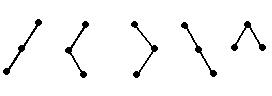
\includegraphics{bintrees}
\end{figure}
\item
Number of sequences of $n$ $X$'s and $n$ $Y$'s such that in any initial segment, the number of $X$'s is at least the number of $Y$'s.
\item
Number of paths from $(0,0)$ to $(n,n)$, that go right or up one unit at each step and that do not go above the main diagonal $y=x$.
\item Number of ways to triangulate a $(n+2)$-gon.
\end{enumerate}
\end{df}
We first derive an identity for the $C_n$.
We claim
\begin{equation}\label{catalanrec}
C_{n+1}=\sum_{k=0}^n C_kC_{n-k}=C_0C_n+C_1C_{n-1}+\cdots+ C_nC_0.
\end{equation}
using any of the definitions. 

To count the number of binary trees with $n+1$ vertices, note that if we take off the root vertex of a tree with $n+1$ vertices, the tree is split into two smaller binary trees, of sizes $k$ and $n-k$, for some $0\le k\le n$. There are $C_kC_{n-k}$ possibilities for these smaller trees. Moreover, this operation is reversible. Thus summing over $0\le k\le n$ gives~(\ref{catalanrec}).

To see the formula holds for the second definition, given a sequence of $X$'s and $Y$'s satisfying the conditions (a {\it ballot sequence}), let $k$ be the smallest nonnegative integer so that there are as many $X$'s as $Y$'s in the first $2(k+1)$ entries. Now delete the first entry and the $2(k+1)$th entry, to get two sequences of lengths $2k$ and $2(n-k)$. The first is a ballot sequence by minimality of $k$ and the second is a ballot sequence since there are as many $X$'s as $Y$'s before the second sequence. The construction is reversible, so we get the same formula as before.

The third definition is equivalent to the second because we can associate taking a step to the right with $X$ and taking a step up as $Y$. The last definition is left to the reader.

Now let $y$ be the generating function for $C_n$. We turn our recurrence relation into an identity involving $f$. $C_{n+1}$ is the coefficient of $x^{n}$ in $\frac{y-1}x$---note we subtract out the constant term before dividing by $x$, so that the result is a power series.
The RHS of~(\ref{catalanrec}), $\sum_{k=0}^n C_kC_{n-k}$, is the coefficient of $x^n$ in $y^2$. Thus using the quadratic formula we get
\begin{align}
\nonumber \frac{y-1}{x}&=y^2\\
\nonumber xy^2-y+1&=0\\
\label{cgfq}y&=\frac{1\pm \sqrt{1-4x}}{2x}.
\end{align}
Now using the binomial formula ($(1+x)^r=\sum_{n=0}^{\iy}\binom rnx^n$ where $\binom rn=\frac{r\fp{n}}{n!}=\frac{r(r-1)\cdots (r-n+1)}{n!}$ we get
\[
\sqrt{1-4x}=(1-4x)^{\rc 2}=\sum_{n=0}^{\iy} \binom{\rc 2}{n} (-4)^nx^n=1-\sum_{n=1}^{\iy}\frac 2n\binom{2(n-1)}{n-1}x^n
\]
since for $n>0$,
\begin{align*}
\binom{\rc2}{n}(-4)^n&=\rc{n!}\pf12\pf{-1}{2}\cdots \pf{-2n+3}{2}(-4)^n=-\rc{n!}2^n(2n-3)(2n-5)\cdots 1\\
&=-\rc{n!}2^n\frac{(2n-2)!}{(2n-2)(2n-4)\cdots 2}=-\frac{2(2(n-1))!}{n!(n-1)!}=-\frac{2}{n}\binom{2(n-1)}{n-1}
\end{align*}
In~(\ref{cgfq}) we take the $-$ sign so that the constant term of the numerator 0 and $y$ is a valid power series. Then
\[
y=\sum_{n=1}^{\iy}\frac{1}{n}\binom{2(n-1)}{n-1}x^{n-1}=\sum_{n=0}^{\iy}\rc{n+1}\binom{2n}{n}x^n.
\]
Hence $C_n=\rc{n+1}\binom{2n}{n}$.
\subsection{Partitions}
One of the most famous generating functions in combinatorics is that of the partition function.
\begin{df}
Let $m$ be a nonnegative integer. 
A \textbf{partition} of $m$ is a way to write it as the sum of positive integers, with order not taken into account. In other words, it is a sequences of positive integers $(\la_1,\ldots, \la_k)$ with $\la_1\ge \cdots \ge \la_k$ and $\sum_{i=1}^k \la_i=m$.

Define $p(n)$ to be the number of partitions of $n$. By convention, $p(0)=1$.
\end{df}

\begin{thm}\label{partitiongf}
The generating function of the sequence $p(n)$ is
\begin{equation}\label{partitiongenfunc}
F(x)=\prod_{n=1}^{\iy}\rc{1-x^n}.
\end{equation}
\end{thm}
\begin{proof}
A partition of $n$ can be specified by a sequence $(a_1,a_2,\ldots)$ where $a_i$ is the number of times $i$ appears in the partition. In order for this to specify a partition of $n$, we must have
\[\sum_{i=1}^n ia_i=n.\]
The number of such sequences $a_i$ is simply the coefficient of $x^n$ in
\[
\prod_{i=1}^{\iy}(1+x^i+x^{2i}+x^{3i}+\cdots )
\]
since each term $x^n$ in the expansion comes from multiplying together terms of the form $x^{ia_i}$, where $x^{ia_i}$ is taken from the $i$th factor in the product above. Using the geometric series formula gives~(\ref{partitiongenfunc}).
\end{proof}
We use the generating function to give an identity for $p(n)$.
\begin{ex}
For a positive integer $m$ let $\si(m)$ denote the sum of divisors of $m$. Then
\[
n\cdot p(n)=\sum_{i=1}^n \si(i)p(n-i).
\]
\end{ex}
\begin{proof}
Note $n\cdot p(n)$ is the coefficient of $x^{n-1}$ in $F'(x)$:
\[
F'(x)=\sum_{n=1}^{\iy}n p(n)x^{n-1}.
\]
Now letting $f_n(x)=\frac{1}{1-x^n}$, we have $F(x)=\prod_{n=1}^{\iy}f_n(x)$. Note
\[
\frac{f_n'}{f_n}
=\frac{nx^{n-1}}{(1-x^n)^2} (1-x^n)=\frac{nx^{n-1}}{1-x^n}
\]
so by logarithmic differentiation\footnote{Note there are infinitely many factors in the product. This is okay, because the coefficient of $x^n$ will be the same in $F'(x)$ as in $(f_1\cdots f_{n+1})'$, so the equation follows from the finite version for each $n$.}
\begin{equation}\label{Fprime}
F'(x)=F(x)\sum_{m=1}^{\iy} \frac{f_m'}{f_m}=F(x)\sum_{m=1}^{\iy}\frac{mx^{m-1}}{1-x^m}.
\end{equation}
\begin{clm}
\[
\sum_{m=1}^{\iy}\frac{mx^{m-1}}{1-x^m}=\sum_{t=1}^{\iy} \si(t)x^{t-1}.
\]
\end{clm}
\begin{proof}
We expand using the geometric series formula and then exchange the order of summation.
\begin{align*}
\sum_{m=1}^{\iy}\frac{mx^{m-1}}{1-x^m}&=\sum_{m=1}^{\iy} mx^{m-1} \sum_{k=0}^{\iy} x^{mk}\\
&=\sum_{m=1}^{\iy} \sum_{k=1}^{\iy} mx^{mk-1}\\
&=\sum_{m>0,\,m\mid t} mx^{t-1}\\
&=\sum_{t=1}^{\iy} \pa{\sum_{m|t} m}x^{t-1}\\
&=\sum_{t=1}^{\iy} \si(t)x^{t-1}.
\end{align*}

What we did above, with less math notation, is just switch from reading the rows to reading the columns of the below sum:\\

\noindent \begin{tabular}{cccccccc}
$\frac{1}{1-x}=$ & $1+$ & $x+$ & $x^{2}+$ & $x^{3}+$ & $x^{4}+$ & $x^{5}+$ & $\cdots$\tabularnewline
$\frac{2x}{1-x^{2}}=$ &  & $2x+$ &  & $2x^{3}+$ &  & $2x^{5}+$ & $\cdots$\tabularnewline
$\frac{3x^{2}}{1-x^{3}}=$ &  &  & $3x^{2}+$ &  &  & $3x^{5}+$ & $\cdots$\tabularnewline
$\frac{4x^{3}}{1-x^{4}}=$ &  &  &  & $4x^{3}+$ &  &  & $\cdots$\tabularnewline
$\frac{5x^{4}}{1-x^{5}}=$ &  &  &  &  & $5x^{4}+$ &  & $\cdots$\tabularnewline
$\frac{6x^{5}}{1-x^{6}}=$ &  &  &  &  &  & $6x^{5}+$ & $\cdots$\tabularnewline
$\vdots$ &  &  &  &  &  &  & $\vdots$\tabularnewline
\hline
 & $\sigma(1)+$ & $\sigma(2)x+$ & $\sigma(3)x^{2}+$ & $\sigma(4)x^{3}+$ & $\sigma(5)x^{4}+$ & $\sigma(6)x^{5}+$ & $\cdots$\tabularnewline
\end{tabular}\\
\end{proof}
Putting the above result into~(\ref{Fprime}) we get
\[
\sum_{n=1}^{\iy} np(n)x^{n-1}=F'(x)=F(x)\sum_{t=1}^{\iy} \si(t)x^{t-1}=\pa{\sum_{n=0}^{\iy} p(n)x^n}
\pa{\sum_{t=1}^{\iy} \si(t)x^{t-1}}.
\]
Matching the coefficients of $x^{n-1}$ on both sides gives the desired result.
\end{proof}

The generating function~(\ref{partitiongenfunc}) for $p(n)$ can in fact be used to obtain much more information about $p(n)$, such as congruences like $p(5n+4)\equiv 0\pmod 5$, and information on its asymptotic growth.
\subsection{Arithmetic progressions}\label{arith}
For some problems we may use apply calculus to get information about the generating functions, such as taking a limit.
\begin{ex}
%%%%%%%%
Suppose the the set of natural numbers is partitioned into arithmetic sequences with first terms $a_1,\ldots, a_k$ and common differences $r_1,\ldots, r_k$, respectively. Then
\begin{enumerate}
\item
$\rc{r_1}+\cdots+\rc{r_k}=1$.
\item
$\frac{a_1}{r_1}+\cdots +\frac{a_k}{r_k}=\frac{k-1}{2}$.
\end{enumerate}
\end{ex}
\begin{proof}
Every natural number occurs in exactly one of the sequences $\{a_1+nr_1\}_{n=0}^{\iy}, \ldots, \{a_k+nr_k\}_{n=0}^{\iy}$, so
\[
\sum_{n=0}^{\iy} x^{a_1+nr_1}+\cdots +\sum_{n=0}^{\iy} x^{a_k+nr_k}=\sum_{n=0}^{\iy} x^n.
\]
Using the geometric series formula, this becomes
\[
\frac{x^{a_1}}{1-x^{r_1}}+\cdots +\frac{x^{a_k}}{1-x^{r_k}}=\rc{1-x}.
\]
This identity holds for $|x|<1$. Multiply through by $1-x$:
\begin{equation}\label{arithseqeq}
\frac{x^{a_1}}{x^{r_1-1}+\cdots +x+1}+\cdots +
\frac{x^{a_k}}{x^{r_k-1}+\cdots +x+1}=1,\quad |x|<1
\end{equation}
Now take the limit as $x\to 1^-$ to get
\begin{equation}\label{aritheq1}
\rc{r_1}+\cdots+\rc{r_k}=1.
\end{equation}
as needed.

To get an identity involving the $a_i$, we differentiate~(\ref{arithseqeq}) to bring the $a_i$ ``out front":
\[
\sum_{i=1}^k \frac{a_ix^{a_i}(x^{r_i-1}+\cdots +1)-x^{a_i}((r_i-1)x^{r_i-2}+\cdots +1)}{(x^{r_i-1}+\cdots +x+1)^2}=0,\quad |x|<1
\]
Now take the limit as $x\to 1^-$:
\[
\sum_{i=1}^k \frac{a_ir_i-\frac{r_i(r_i-1)}{2}}{r_i^2}=-\frac k2+\sum_{i=1}^{\iy} \pa{\frac{a_i}{r_i}+\rc{2r_i}}=0.
\]
Now use~(\ref{aritheq1}) to get
\[
\sum_{i=1}^k \frac{a_i}{r_i}=\frac{k-1}{2}.
\]
\end{proof}
\subsection{Extracting coefficients}
In this section we consider generating functions which are polynomials. 
Sometimes, rather than finding a specific coefficient, we want to find a sum of coefficients, for instance the sum of coefficients of $x^n$ with $n$ divisible by $k$. To do this, we evaluate the polynomial at the $k$th roots of unity and take the average.\footnote{For background on complex numbers see lecture 11, \url{http://onlinemathcircle.com/wp-content/uploads/2011/02/10-complex.pdf}}
\begin{lem}\label{extcoef}
Let $\om=e^{\frac{2\pi i}{k}}$. Then the sum of the coefficients of $x^n$ with $k|n$ in the polynomial $P(x)$ is
\[
\frac{P(1)+P(\om)+\cdots +P(\om^{k-1})}{k}.
\]
\end{lem}
\begin{proof}
For a $k$th root of unity $\zeta$,
\[1+\zeta+\cdots +\zeta^{k-1}=\begin{cases}
0,&\zeta\ne 1\\
k,&\zeta=1.
\end{cases}\]
If $P(x)=\sum_{n=0}^{\iy} a_nx^n$, the the contribution to the sum $P(1)+P(\om)+\cdots +P(\om^{k-1})$ from the $x^n$ terms is $a_n(1+\om^n+\cdots +\om^{n(k-1)})$, which by the above, is $a_nk$ when $\om^n=1$ i.e. $k|n$, and 0 otherwise.
\end{proof}
(Query: Given $r$, how would you find the sum of coefficients of $x^n$ with $n\equiv r\pmod{k}$?)

A quick example: Suppose we want to find the number of subsets of an $n$-element subset with number of elements divisible by 3. This is just the sum of the coefficients of $x^i$ (which are binomial coefficients $\binom ni$) for $3|i$, in $(1+x)^n$. Using Lemma~\ref{extcoef} and letting $\om=\frac{-1+\sqrt 3 i}{2}$ be the third root of unity, the answer is
\[
\frac{2^n+(1+\om)^n+(1+\om^2)^n}{3}=\frac{2^n+\pf{1+\sqrt 3i}{2}^n+\pf{1-\sqrt 3i}{2}^n}{3}.
\]

Now for something more hardcore.
\begin{ex}[IMO 1995/6]\label{imo95-6}
Let $p>2$ be a prime number and let $A=\{1,2,\ldots, 2p\}$. Find the number of subsets of $A$ having $p$ elements and having sum of elements divisible by $p$.
\end{ex}
\noindent {\it Solution.}
Consider the generating function
\[
(1+x)(1+x^2)\cdots (1+x^{2p}).
\]
The coefficient of $x^i$ in the expansion is the number of subsets of $A$ whose sum of elements is $i$. Indeed, each subset of $A$ is associated with a term in the expansion, by taking 1 from the $i$th term if $i\nin A$, and $x^i$ from the $i$th term if $i\in A$.

Consider the generating function
\[
\underbrace{(1+y)(1+y)\cdots (1+y)}_{2p}.
\]
The coefficient of $y^j$ in the expansion is the number of subsets of $A$ with $j$ elements. Indeed, each subset of $A$ is associated with a term in the expansion, by taking 1 from the $j$th term if $j\nin A$, and $y$ from the $j$th term if $j\in A$.

But we want information about both the number of elements in the subset and the sum of the elements in the subset, at the {\it same time}. What do we do? Put the two together! Consider the generating function
\[
P(x,y)=(1+xy)(1+x^2y)\cdots (1+x^{2p}y).
\]
The coefficient of $x^iy^j$ is the number of subsets of $A$ with $j$ elements with sum of elements equal to $i$. Think of the variables $x$ and $y$ as being counters for different things.

For example, in the case of $p=3$, the term $xy\cdot 1\cdot x^3y\cdot 1\cdot x^5y\cdot 1=x^9y^3$ corresponds to the subset $\{1,3,5\}$.

Thus we want the sum of the coefficients of $x^iy^p$ where $p|i$. Treating $P(x,y)$ as a polynomial in $x$ and applying Lemma~\ref{extcoef}, we want the coefficient of $y^p$ in
\begin{equation}\label{imo95-6-1}
\frac{P(1,y)+P(\om, y)+\cdots +P(\om^{p-1},y)}{p},\quad \om=e^{\frac{2\pi i}{p}}.
\end{equation}
Note for $\zeta\neq 1$ a $p$th root of unity, $1,\zeta,\ldots, \zeta^{p-1}$ runs through all $p$th roots of unity and hence $t^p-1=(t-1)(t-\zeta)\cdots (t-\zeta^{p-1})$. Then
\begin{align*}
P(\zeta,y)&=[(1+\zeta y)\cdots (1+\zeta^py)][(1+\zeta^{p+1}y)\cdots (1+\zeta^{2p}y)]\\
&=[(1+\zeta y)\cdots (1+\zeta^py)]^2\\
&=y^{2p}[(-y^{-1}-\zeta)\cdots (-y^{-1}-\zeta^p)]^2\\
&=y^{2p}[(t^p-1)|_{t=-y^{-1}}]^2\\
&=(y^p+1)^2.
\end{align*}
When $\zeta=1$,
\[P(\zeta,y)=(y+1)^{2p}.\]
Putting these two cases together,
\[
\frac{P(1,y)+\cdots +P(\om^{p-1},y)}{p}=\frac{(y+1)^{2p}+(p-1)(y^p+1)^2}{p}.
\]
The coefficient of $y^p$ is
\[
\frac{\binom{2p}{p}+2(p-1)}{p}
\]
which is the answer.

\section{Problems}
\begin{enumerate}
\item Find the generating function for the Fibonacci numbers, defined by $F_0=0$, $F_1=1$ and $F_{n+2}=F_n+F_{n+1}$ for $n\ge 0$. Then simplify the following (i.e. write it as an expression involving only a fixed number of $F_i$'s):
\begin{enumerate}
\item $\sum_{i=0}^n F_i$
\item $\sum_{i=0}^{n-1} F_{2i+1}$
\item $\sum_{i=0}^n F_{2i}$
\item $\sum_{i=0}^n iF_i$
\item $\sum_{i=0}^n F_iF_{n-i}$
\end{enumerate}
\item Given that $\{a_n\}_{n=0}^{\iy}$ satisfies $\sum_{i=0}^n a_np^{n-i}=b_n$ for each integer $n$, find $a_n$ in terms of $n$ and $b_n$. Same problem, for $\sum_{i=0}^n a_n(n-i)p^{n-i}=b_n$.
\item 
Let
\[
(1+x+x^2+\cdots +x^8)^{100}=\sum_{n=0}^{800} a_n x^n.
\]
Find $\sum_{n=0}^{800} na_n$.
\item Prove that $\sum_{n=0}^m \binom{n+k}{k}=\binom{n+m+1}{k+1}$.
\item Given $n\in\N_0$, find the number of $k$-tuples of nonnegative integers $(a_1,\ldots, a_k)$ such that $a_1+\cdots +a_k=n$.
\item Let $n>1$ and consider a fair die $D$ with $n^2$ faces, labeled $1,2,\ldots, n^2$. Prove that there exists two dice $A$ and $B$, different from $D$, each with $n^2$ faces labeled by positive integers, such that the probability distribution of the sum of two rolls of $D$ is the same as the probability distribution of the sum of one roll of $A$ and one roll of $B$.
\item Let $b_n$ be the number of ways to write $n$ as a sum of nonnegative integer powers of 2.
\begin{enumerate}
\item
Find the generating function for $b_n$.
\item
Prove that
\[
b_n=\sum_{i=0}^{\fl{\frac n2}} b_i.
\]
Try to find both a combinatorial and a generating function proof, for comparison.
\end{enumerate}
\item Let $a_n$ denote the number of ways to tile a $3\times n$ board with dominoes. Find a generating function for $a_n$, then give an explicit formula. (Note: you need to have two generating functions for this problem. One is for $a_n$; one is for the $b_n$, the number of ways to tile a $3\times n$ rectangle with one corner missing.)
\item Five people stand at the vertices of a pentagon, throwing frisbees to each other. At time 0, two people at adjacent vertices have the frisbees, and in each time interval, each frisbee is thrown to the left or right with probability $\rc2$. This process continues until one person receives two frisbees simultaneously. Let $p_n$ be the probability that the game ends after exactly $n$ steps.
\begin{enumerate}
\item
Find a generating function for $p_n$. (As in the previous problem, set up a system of equations involving generating functions.)
\item
Find $p_n$.
\item
Find the expected number of steps until the game ends ($\sum_{n=0}^{\iy} np_n$). Hint: differentiate. (This problem shows how generating functions can be useful in probability. See~\cite[\S 8.4]{gkp} for a cool application of generating functions to coin-flipping games.)
\end{enumerate}

\item (AwesomeMath Team Contest 2008, David Rush) If any element of the set \[\{0,1,\ldots, m^3-1\}\] is considered a digit in modified base $m$, prove that, for all positive integers $n$ the number of modified base $m$ representations of $n$ is an integer multiple of $\frac{\fl{\frac{n}{m^2}}+1}{2}$.

\item Show that the number of partitions of $n$ into odd parts equals the number of partitions of $n$ into distinct parts.

\item (IMO 2008/5) Let $n$ and $k$ be positive integers with $k\ge n$ and $k-n$ an even number. Let $2n$ lamps labelled $1,2,\ldots, 2n$ be given, each of which can be either {\it on} or {\it off}. Initially all the lamps are off. We consider a sequence of {\it steps}: at each step one of the lamps is switched (from on to off or from off to on).

Let $N$ be the number of such sequences consisting of $k$ steps and resulting in the state where lamps 1 through $n$ are all on, and lamps $n+1$ through $2n$ are all off.  Let $M$ be the number of such sequences consisiting of $k$ steps and resulting in the state where lamps 1 through $n$ are all on, and lamps $n+1$ through $2n$ are all off, but where none of the lamps $n+1$ through $2n$ is ever switched on.

Determine the ratio $N/M$.
\item Suppose that the natural numbers are written as a disjoint union of arithmetic progressions with differences $d_1\ge d_2\ge\cdots \ge d_n$. Show $d_1=d_2$.
\item (Euler's pentagonal number theorem) Prove that
\[
\prod_{n=1}^{\iy}(1-x^n)=\sum_{k\in\Z} (-1)^k x^{k(3k-1)/2}=1-x-x^2+x^5+x^7-x^{12}-x^{15}+\cdots.
\]
Conclude that
\[
p(n)=\sum_{k\in  \Z}(-1)^{k-1}p\pa{n-\frac{k(3k-1)}{2}}.
\]
(Hint: One way to proceed is to distribute the $(1-x)$ in each term, then distribute the $(1-x^2)$, and so on; proceed by induction after coming up with a suitable statement in terms of $k$. Combinatorial approaches are also possible.)
\item Show that 
\[
\prod_{n=1}^{\iy} \rc{1-x^n}=1+\sum_{m=1}^{\iy} \frac{x^{m^2}}{(1-x)^2(1-x^2)^2\cdots (1-x^m)^2}.
\]
(Hint: Given a partition, its corresponding {\it Ferrers diagram} is a left-justified array of dots with $k$ rows, where there are $\la_i$ dots in the $i$th row. The {\it Durfee square} of a Ferrers diagram is the largest square of dots, at the upper left hand corner of the diagram. How does the Durfee square split up the Ferrers diagram?)
%The Durfee square divides a partition into a perfect square and two smaller partitions.
\item (AwesomeMath Team Contest 2010, Brian Basham)
Fatty McButterpants is bored and decides to toss stones into two buckets. Both buckets start with no stones, and every second he throws a stone into the first bucket, the second bucket, or no buckets, each with probability $\frac{1}{3}$. After $n$ seconds, what is the probability that the number of stones in each bucket is divisible by $3$?
\item (Mathematical Reflections, O107) Let $p_1,p_2,p_3$ be distinct primes and let $n$ be a positive integer. Find the number of functions $f:\{1,2,\ldots, 2n\}\to \{p_1,p_2,p_3\}$ for which $f(1)f(2)\cdots f(2n)$ is a perfect square.
\item How many subsets of $\{1,2,\ldots, 2000\}$ have sum of elements divisible by 5?
\item Let $p$ and $q$ be distinct primes greater than 2. How many subsets of size $pq$ in $\{1,2,\ldots, 2pq\}$ have sum divisible by $pq$?
\item (ISL 2002/A5) Let $m$ and $n$ be integers greater than 1 and let $a_1,\ldots, a_n$ be integers, none of which is divisible by $m^{n-1}$. Prove that we can find integers $e_1,\ldots, e_n$, not all zero, such that $|e_i|<m$ for all $i$ and $m^n|e_1a_1+\cdots +e_na_n$.

\item (Putnam 1992) For nonnegative integers $n$ and $k$, define $Q(n,k)$ to be the coefficient of $x^k$ in the expansion of $(1+x+x^2+x^3)^n$. Prove that
\[
Q(n,k)=\sum_{j=0}^n\binom nj \binom{n}{k-2j}.
\]
\item (Putnam 1997/B4) Let $a_{m,n}$ denote the coefficient of $x^n$ in the expansion of $(1+x+x^2)^m$. Prove that for all $k\ge 0$,
\[
0\le \sum_{i=0}^{\fl{2k/3}} (-1)^i a_{k-i,i}\le 1.
\]
\item (Putnam 1999/B3) Let $A=\{(x,y):0\le x,y< 1\}$. For $(x,y)\in A$, let
\[S(x,y)=\sum_{\rc 2\le \frac mn\le 2} x^my^n,\]
where the sum ranges over all pairs $(m,n)$ of positive integers satisfying the indicated inequalities. Evaluate
\[
\lim_{(x,y)\to 1,(x,y)\in A} (1-xy^2)(1-x^2y)S(x,y).
\]
\item (Putnam 2003/A6) For a set $S$ of nonnegative integers, let $r_S(n)$ denote the number of ordered pairs $(s_1,s_2)$ such that $s_1\in S,s_2\in S,s_1\ne s_2$, and $s_1+s_2=n$. Is it possible to partition the nonnegative integers into two sets $A$ and $B$ in such a way that $r_A(n)=r_B(n)$ for all $n$?
\item (Putnam 2005/B4) For positive integers $m$ and $n$, let $f(m,n)$ denote the number of $n$-tuples $(x_1,\ldots, x_n)$ of integers such that $|x_1|+\cdots +|x_n|\le m$. Show that $f(m,n)=f(n,m)$.
\item Start with a finite number of chips placed on the integers on a number line; suppose $c_i$ chips are placed on $i$. 
 Let $m$ and $n$ be positive integers such that $n>m$. 
At each step, we may remove $m+n$ chips from an integer $i$ and place $1$ chip on $i+1$ and $mn$ chips on $i-1$. Suppose for each integer $i$, there is a time after which the number of chips on $i$ is constant. Let $d_i$ be this constant.
Prove that
\[
\sum_{i\in \Z} c_i n^i=\sum_{i\in \Z}d_i n^i.
\]
Is this true for $n$ replaced by $m$?

\end{enumerate}
\section{Appendix}
%\begin{align*}
%\sum_{k=0}^{\iy} {r^k} x^k&=\rc{1-rx}\\
%\sum_{k=0}^{\iy} {r^k} x^k&=\rc{1-rx}\\
%\sum_{k=0}^n {\binom nk} x^k&=(1+x)^n&n\in \N\\
%\sum_{k=0}^{\iy} {\binom rk}x^k&=(1+x)^r&r\in \R\\
%\sum_{k=0}^{\iy}\rc{1}{k!}{x^k} &=e^x\\
%\sum_{k=0}^{\iy} (-1)^k\rc{(2k)!}x^k&=\cos x\\
%\sum_{k=0}^{\iy} (-1)^k \rc{(2k+1)!}x^k&=\sin x\\
%\sum_{k=0}^{\iy} \rc{(2k)!}x^k&=\cosh x=\frac{e^x+e^{-x}}2\\
%\sum_{k=0}^{\iy} \rc{(2k+1)!}x^k&=\sinh x=\frac{e^x-e^{-x}}2\\
%\sum_{k=0}^{\iy} (n+1)x^n&= \rc{(1-x)^2}
%\end{align*}
Note the definition
\[
\binom mn=\frac{m\fp{n}}{n!}=\frac{m(m-1)\cdots (m-n+1)}{n!},\,m\in \R,n\in \N_0.
\]

\noindent \begin{tabular}{|c|c|c|}
\hline 
Sequence & Generating function & Closed form\tabularnewline
\hline 
$1,1,1,\ldots$ & $\displaystyle\sum_{n=0}^{\infty}x^{n}$ & $\displaystyle\frac{1}{1-x}$\tabularnewline
\hline 
$1,-1,1,\ldots$ & $\displaystyle\sum_{n=0}^{\infty}(-1)^{n}x^{n}$ & $\displaystyle\frac{1}{1+x}$\tabularnewline
\hline 
$1,r,r^{2},\ldots$ & $\displaystyle\sum_{n=0}^{\infty}r^{n}x^{n}$ & $\displaystyle\frac{1}{1-rx}$\tabularnewline
\hline 
$\displaystyle \underbrace{1,0,\ldots,0}_{k}1,0,\ldots,1,\ldots$ & $\displaystyle\sum_{n=0}^{\infty}x^{nk}$ & $\displaystyle\frac{1}{1-x^{k}}$\tabularnewline
\hline 
$\displaystyle \binom{m}{0},\binom{m}{1},\ldots,\binom{m}{m}$, $ m\in\N$ & $\displaystyle\sum_{n=0}^{m}\binom{m}{n}x^{n}$ & $\displaystyle (1+x)^{m}$\tabularnewline
\hline 
$\displaystyle\binom{r}{0},\binom{r}{1},\binom{r}{2}\ldots$, $\displaystyle r\in\R$ & $\displaystyle \sum_{n=0}^{\infty}\binom{r}{n}x^{n}$ & $\displaystyle (1+x)^{r}$\tabularnewline
\hline 
$\displaystyle \binom{r}{r},\binom{r+1}{r},\binom{r+2}{r},\ldots$ & $\displaystyle \sum_{n=0}^{\infty}\binom{r+n}{r}x^{n}$ & $\displaystyle \frac{1}{(1-x)^{r}}$\tabularnewline
\hline 
$\displaystyle 1,\frac{1}{1!},\frac{1}{2!},\frac{1}{3!},\ldots$ & $\displaystyle \sum_{n=0}^{\iy}\frac{1}{n!}x^{n}$ & $\displaystyle e^{x}$\tabularnewline
\hline 
$\displaystyle 1,0,-\frac{1}{2!},0,\frac{1}{4!},\ldots$ & $\displaystyle \sum_{n=0}^{\iy}\frac{(-1)^{n}}{(2n)!}x^{2n}$ & $\displaystyle \cos x$\tabularnewline
\hline 
$\displaystyle 0,\frac{1}{1!},0,-\frac{1}{3!},\ldots$ & $\displaystyle \sum_{n=0}^{\iy}\frac{(-1)^{n}}{(2n+1)!}x^{2n+1}$ & $\displaystyle \sin x$\tabularnewline
\hline 
$\displaystyle 1,0,\frac{1}{2!},0,\frac{1}{4!},\ldots$ & $\displaystyle \sum_{n=0}^{\iy}\frac{1}{(2n)!}x^{2n}$ & $\displaystyle \cosh x=\frac{e^{x}+e^{-x}}{2}$\tabularnewline
\hline 
$\displaystyle 0,\frac{1}{1!},0,\frac{1}{3!},\ldots$ & $\displaystyle \sum_{n=0}^{\iy}\frac{1}{(2n+1)!}x^{2n+1}$ & $\displaystyle \sinh x=\frac{e^{x}-e^{-x}}{2}$\tabularnewline
\hline 
$\displaystyle 0,1,-\frac{1}{2},\frac{1}{3},-\frac{1}{4},\ldots$ & $\displaystyle \sum_{n=1}^{\iy}\frac{(-1)^{n-1}}{n}x^n$ & $\displaystyle \ln(1+x)$\tabularnewline
\hline
\end{tabular}\\

Let $f(x)=\sum_{n=0}^{\iy} a_nx^n$, $g(x)=\sum_{n=0}^{\iy} b_nx^n$.

\noindent \begin{tabular}{|c|c|}
\hline 
Sequence & Generating function\tabularnewline
\hline 
$ca_{n}+b_{n}$ & $cf+g$\tabularnewline
\hline 
$a_{n-m}$ & $x^{m}f$\tabularnewline
\hline 
$a_{n+m}$ & $\displaystyle \frac{f-a_{m-1}x^{m-1}-\cdots-a_{0}}{x^{m}}$\tabularnewline
\hline 
$c^{n}a_{n}$ & $f(cx)$\tabularnewline
\hline 
$a_{n/m}$ (0 if $m\nmid n$) & $f(x^{m})$\tabularnewline
\hline 
$(n+1)a_{n+1}$ & $f'$\tabularnewline
\hline 
$na_{n}$ & $xf'$\tabularnewline
\hline 
$a_{n}b_{0}+\cdots+a_{0}b_{n}$ & $fg$\tabularnewline
\hline 
$a_{0}+\cdots+a_{n}$ & $\displaystyle \frac{1}{1-x}f$\tabularnewline
\hline 
$\displaystyle \frac{a_{n-1}}{n},\, n\ge1$ & $\displaystyle \int_{0}^{x}f(u)\, du$\tabularnewline
\hline
\end{tabular}
%TODO: Add table of manipulating series
\begin{thebibliography}{9}
\bibitem{PftB} Andreescu, T.; Dospinescu, G.: {\it Problems from The Book}. XYZ Press, Allen TX, 2008.
\bibitem{gkp} L. Graham, D. Knuth, and O. Patashnik. {\it Concrete Mathematics: A Foundation for Computer Science}. Addison-Wesley, 1989.
\bibitem{fs} P. Flajolet and R. Sedgewick. {\it Analytic Combinatorics}. Cambridge University Press, 2009. \url{http://algo.inria.fr/flajolet/Publications/book.pdf}.

\bibitem{wilf} H. Wilf. {\it generatingfunctionology}. Academic Press, Inc., 1994. 
\url{http://www.math.upenn.edu/~wilf/gfologyLinked2.pdf}

\bibitem{yuan} Q. Yuan. Topics in Generating Functions, 2009.  \url{http://web.mit.edu/~qchu/Public/TopicsInGF.pdf}
\end{thebibliography}
\end{document}